\documentclass{article}

\usepackage{lipsum}
\usepackage[margin=1in,includefoot]{geometry}
\usepackage{graphicx}
\usepackage{float}
\usepackage[hidelinks]{hyperref}

% Header and Footer Stuff
\usepackage{fancyhdr}
\pagestyle{fancy}
\fancyhead{}
\fancyfoot{}
\fancyfoot[R]{\thepage}
\renewcommand{\headrulewidth}{0pt}
\renewcommand{\footrulewidth}{0pt}

\begin{document}

\begin{titlepage}
	\begin{center}
	\line(1,0){300}\\
	[0.25in]
	\huge{\bfseries The Bipolar Junction Transistor Inverter}\\
	[2mm]
	\line(1,0){200}\\
	[1.5cm]
	\textsc{\LARGE Laboratory D1 }\\
	[0.75cm]
	\textsc{\Large 3C2 Digital Circuits}\\
	[9cm]	
	\end{center}
	
	\begin{flushright}
	\textsc{\large Alexandru Sulea\\
	D Stream\\
	\#12315152\\
	27 October 2015\\}
	\end{flushright}

\end{titlepage}
%Table of Contents Stuff%
\tableofcontents
\listoffigures
\addcontentsline{toc}{section}{List of Figures}
\listoftables
\addcontentsline{toc}{section}{List of Tables}


\thispagestyle{empty}
\cleardoublepage
\pagenumbering{arabic}
\setcounter{page}{1}


\section{Introduction}\label{sec:intro}
The purpose of the D1 laboratory is to examine the properties and functions of a Bipolar Junction Transistor. The experiments will encompass the topics covered in the 3C2 Digital Circuits lectures. The lab also serves as an introduction to designing circuits encompassing Bipolar Junction transistors in Multisim.

\section{Theory}\label{sec:theory}

A bipolar transistor is comprised of three layers of differently doped semiconductor materials
Constructing P-N-P or N-P-N transistors. \\
Bipolar transistors are named as such due to their operation involving holes and electrons. Electrons are majority charge carriers in N-type semiconductors, whereas holes are majority charge carriers in P-type semiconductors. 


\subsection{A:Bipolar Junction Transistor Characteristics}
A bipolar junction transistor is a type of transistor that relies on the contact of two types of semiconductor for its operation. There are two types of BJT transistors, NPN and PNP.\\
In an NPN transistor, a thin and lightly doped P-type base is sandwiched between a heavily doped N-type emitter and another N-type collector;
 In a PNP transistor, a thin and lightly doped N-type base is sandwiched between a heavily doped P-type emitter and another P-type collector.(Ref.1)\\
NPN transistors are much more
popular than PNP transistors because electrons move faster in a semiconductor. As a results,
a NPN transistor has a faster response time compared to a PNP transistor.
BJTs can be found either as individual discrete components, or in large numbers as parts of integrated circuits. BJTs can be used as amplifiers, switches, or in oscillators.(Ref.2)\\



\subsection{B:Resistevely Loaded BJT Inverter Characteristics}
The BJT modes of operation are easily found due to the fact that it can only be in three modes, cut-off, forward active and saturated. These two factors of easy modifiability and easy steps to find its mode of operation make the BJT a very useful inverter.\\

Varying various components and characteristics of the BJT inverter can adversely change the voltage transfer characteristics. The resistor values of Rb and Rc change both the slope of the Vi and the ending Vol. Increasing the value of Rb decreases the slope of the Vil and increases the Vol, whereas decreasing Rb increases the slope of the VTC and decreases Vol. Increasing Rc does the opposite of increasing Rb, it increases the slope and lowers the Vol, decreasing Rc does the opposite. Decreasing the Bf alters the slope of the Vil only by decreasing it, while an increase makes the Vil drop faster.(Ref.6)

The BJT inverter is a very stable inverter and adjusting its Vil is relatively simple. By simply changing the resistor values, one can attain a desired Vil and obtain desired critical voltages. 

\subsection{C:BJT Inverter Switching Performance}
In an electronic circuit there are no mechanical switches. The switching action itself is performed by a transistor with an input voltage (Pic. 8).In a switching operation a transistor is usually controlled in two condition states, which can be referred to as loosly as the "on" state and the "off" state. A switch should appear as a short circuit when turned on and an open circuit when turned off.(Ref.5)
Although the BJT can be made to act as a switch it technically isn't one in a mechanical sense but it servers as a useful replacement. Since it is not a mechanical switch it is desirable to always switch from one state to the other as quickly as possible with little loss time in between. 




\pagebreak


\section{Results}\label{sec:result}

\subsection{A:Bipolar Junction Transistor Characteristics}


\subsubsection{A1:Collector Current against Base - Emitter Voltage}
\begin{figure}[H]
	\centering
	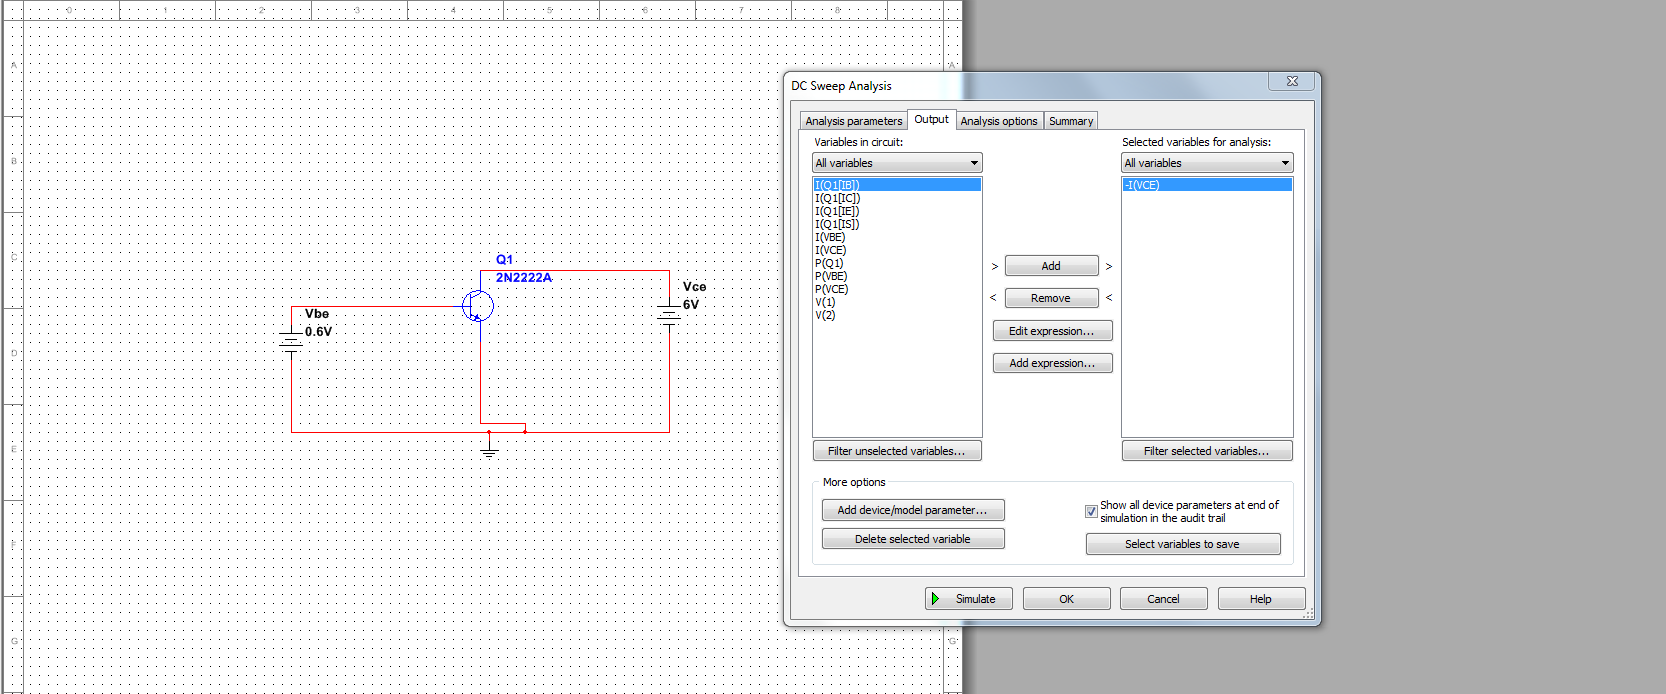
\includegraphics[height=3in]{/home/owner/Desktop/LAB REPORTS/D1/Pic1.PNG}
	\caption[A.1 electronic set-up]{A.1 Part.9}
	\label{fig:pic}
\end{figure}
Figure \ref{fig:pic} Shows the initial set up

\begin{table}[H]

	\centering
	\label{tab:firstTable}
	\caption[A.1 Part.4 Table]{A.1 Part.4 }
	                  
	\begin{tabular}{lcr}
		BF, the foreward active current 
		gain(Bf)&220 \\ \hline 
		BR, the foreward active current
		gain(Br)&4\\ \hline
		TF,the foreward transit time(Tf)
		&0.325E-9s\\ \hline
		TR,the reverse transit time(Tf)
		&100E-9s\\ \hline
		CJC,B-C zero-bias depletion capacitance
		(Cbc)&9.12E-12F\\ \hline
		CJE,B-E zero-bias depletion capacitance
		(Cbe)&27.01E-12F\\ \hline
		

	\end{tabular}
\end{table}

Table \ref{tab:firstTable} Completed from the given values

\begin{figure}[H]
	\centering
	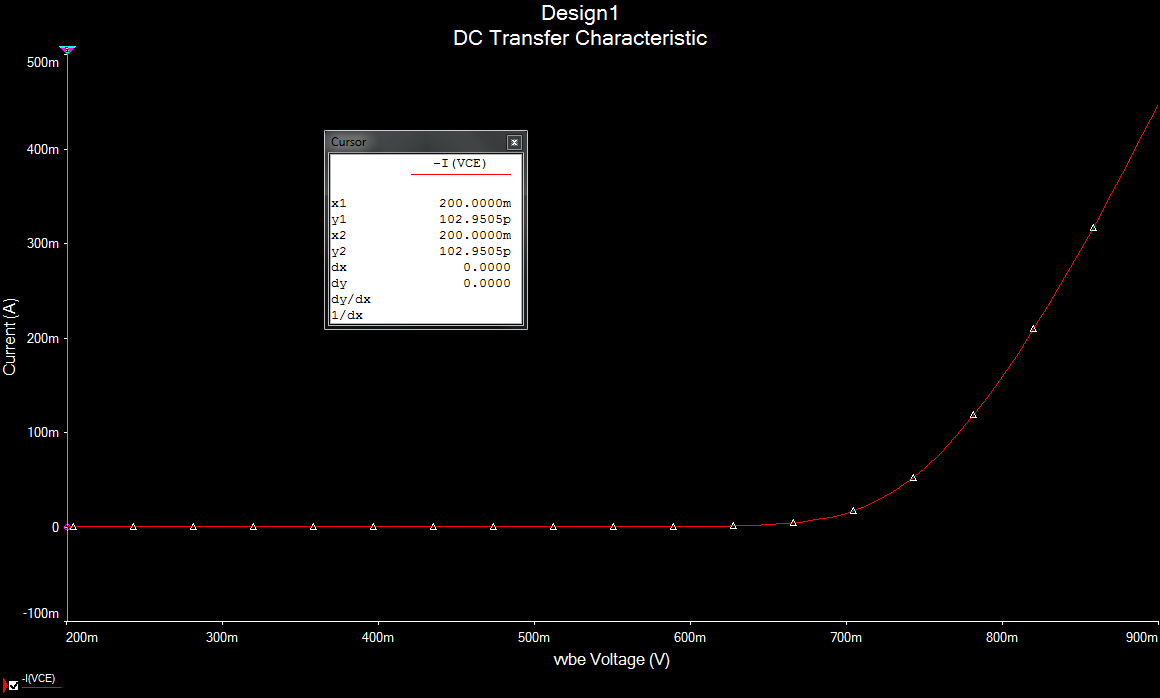
\includegraphics[height=3in]{/home/owner/Desktop/LAB REPORTS/D1/Pic2.PNG}
	\caption[A.1 Part.12 Plot ]{A.1 Part.12}
	\label{fig:pic}
\end{figure}

\begin{table}[H]

	\centering
	\label{tab:secondTable}
	\caption[A.1 Part.13 Table]{A.1 Part.13}
	\begin{tabular}{lcr}
	Vbe cut-in&0.770V \\ \hline
	Vbe on&0.670V\\ \hline
		
	\end{tabular}
\end{table}

\begin{figure}[H]
	\centering
	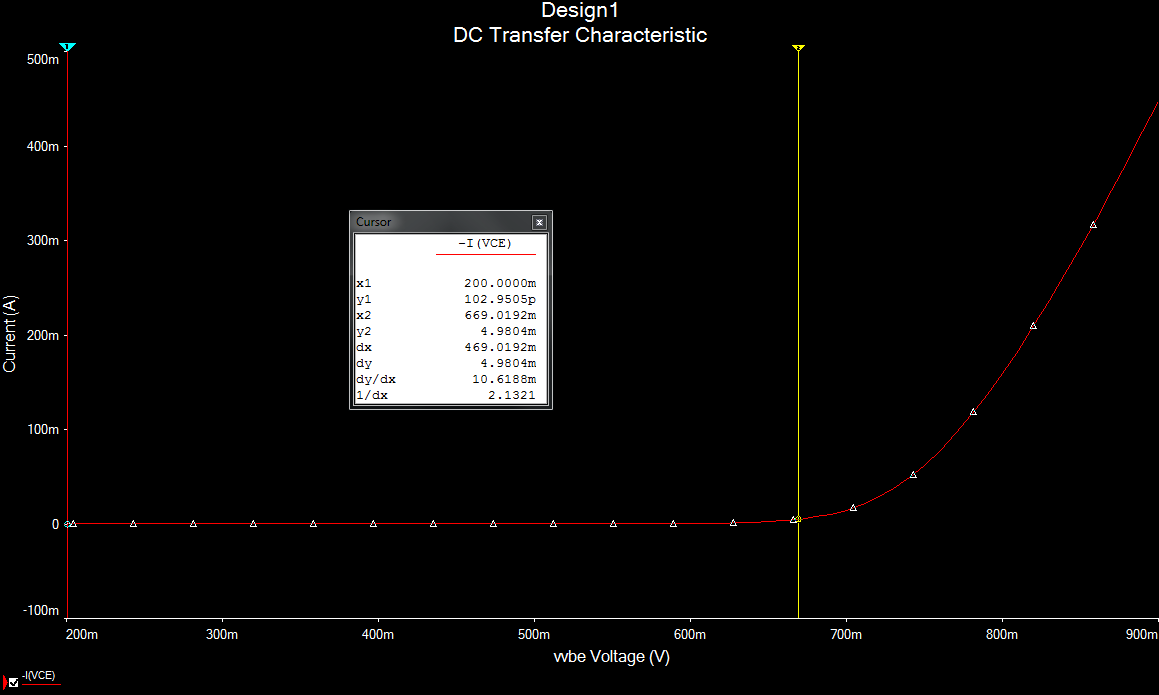
\includegraphics[height=3in]{/home/owner/Desktop/LAB REPORTS/D1/pic3.PNG}
	\caption[A.1 Part.13 Plot]{A.1 Part.13}
	\label{fig:pic}
\end{figure}
\pagebreak

A.1 Part.13
Q. How do the values of Vbe cut-in and Vbe on compare with those in lectures?\\
Ans. The values in the lectures are mostly ideal. Here we see a gradual increase in the value and a more realistic curve.

\subsubsection{A2:Collector Current vs. Collector-Emitter Voltage}

\begin{figure}[H]
	\centering
	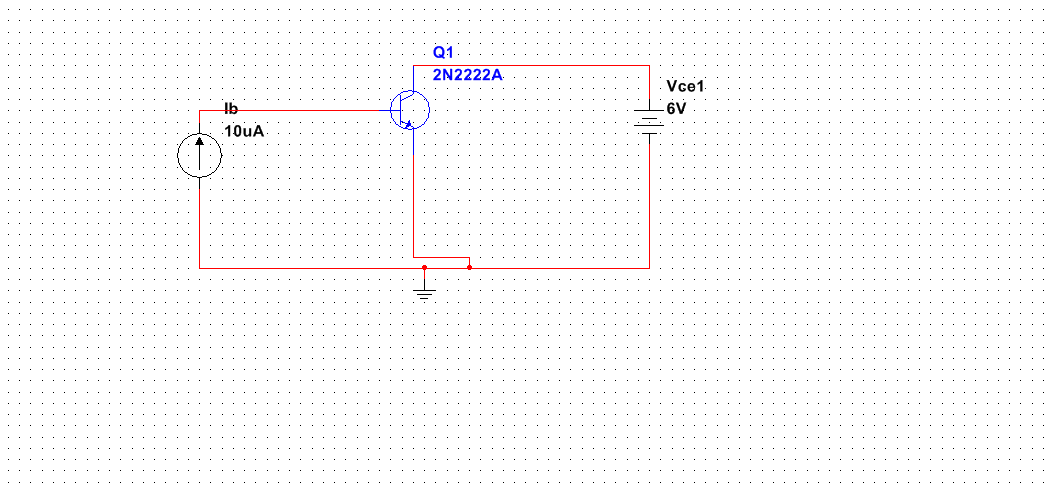
\includegraphics[height=3in]{/home/owner/Desktop/LAB REPORTS/D1/Pic4.PNG}
	\caption[A.2 electronic set-up]{A.2 Part.1}
	\label{fig:pic}
\end{figure}


\begin{table}[H]
	\centering
	\label{tab:thirdTable}
	\caption[A.2 Part.5 Plot values Table]{A.2 Part.5}
	\begin{tabular}{lcr}
		Bf@Ib=10uA&2500 \\ \hline
		Bf@Ib=100uA&210\\ \hline
		Vcesat@Ic=5mA&0.25V\\ \hline
	\end{tabular}
\end{table}

\begin{figure}[H]
	\centering
	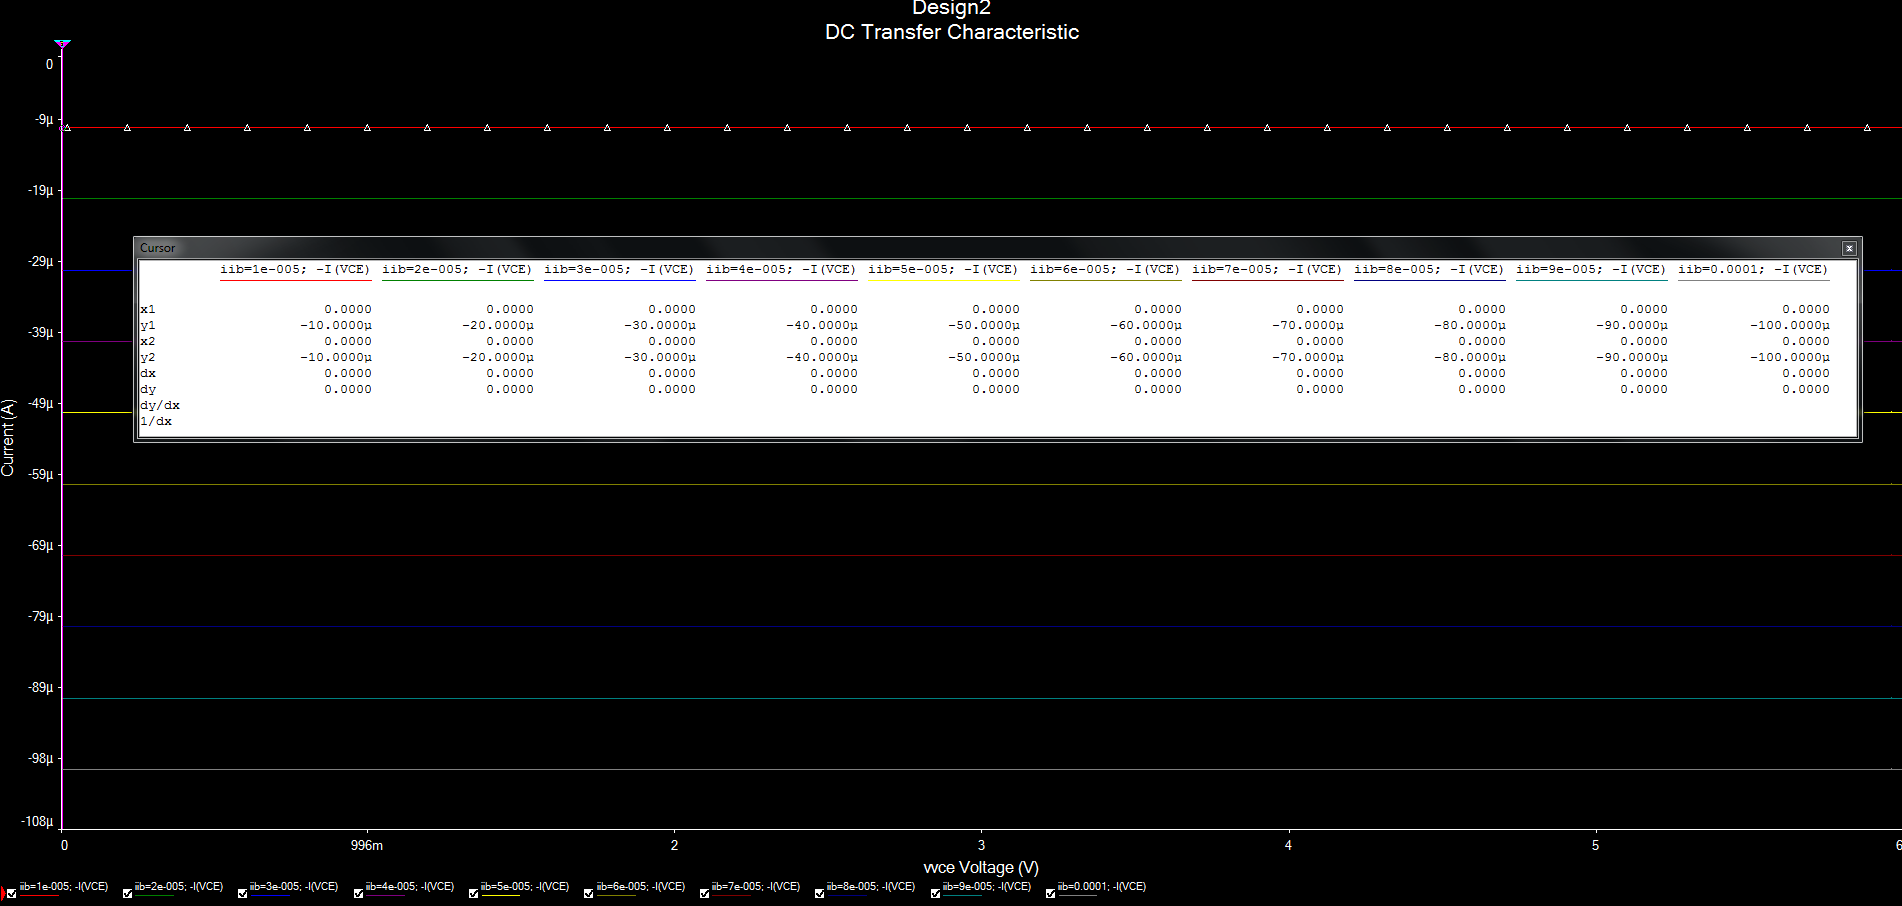
\includegraphics[height=3in]{/home/owner/Desktop/LAB REPORTS/D1/Pic5.PNG}
	\caption[A.2 Part.5 Plot]{A.2 Part.5}
	\label{fig:pic}
\end{figure}

\begin{figure}[H]
	\centering
	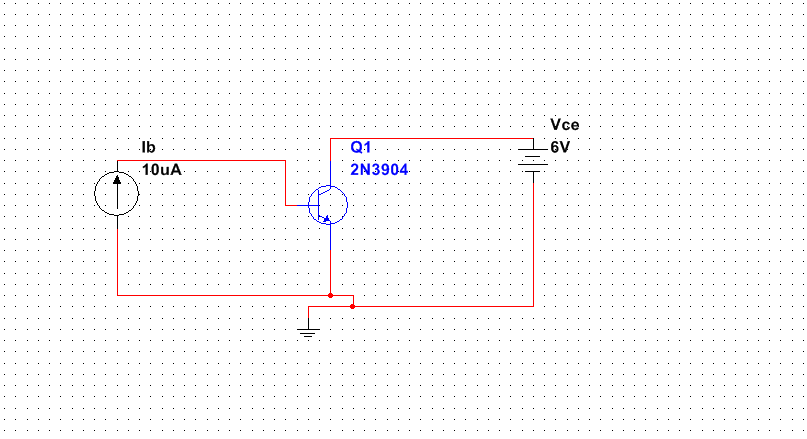
\includegraphics[height=3in]{/home/owner/Desktop/LAB REPORTS/D1/Pic6.PNG}
	\caption[A.2 Part.6 electronic set-up]{A.2 Part.6}
	\label{fig:pic}
\end{figure}

\begin{table}[H]
	\centering
	\label{tab:fourthTable}
	\caption[A.2 Part.6 Plot Values Table]{A.2 Part.6}
	\begin{tabular}{lcr}
		Bf@Ib=10uA&140 \\ \hline
		Bf@Ib=100uA&160\\ \hline
		Vcesat@Ic=5mA&0.22V\\ \hline
	\end{tabular}
\end{table}


\begin{figure}[H]
	\centering
	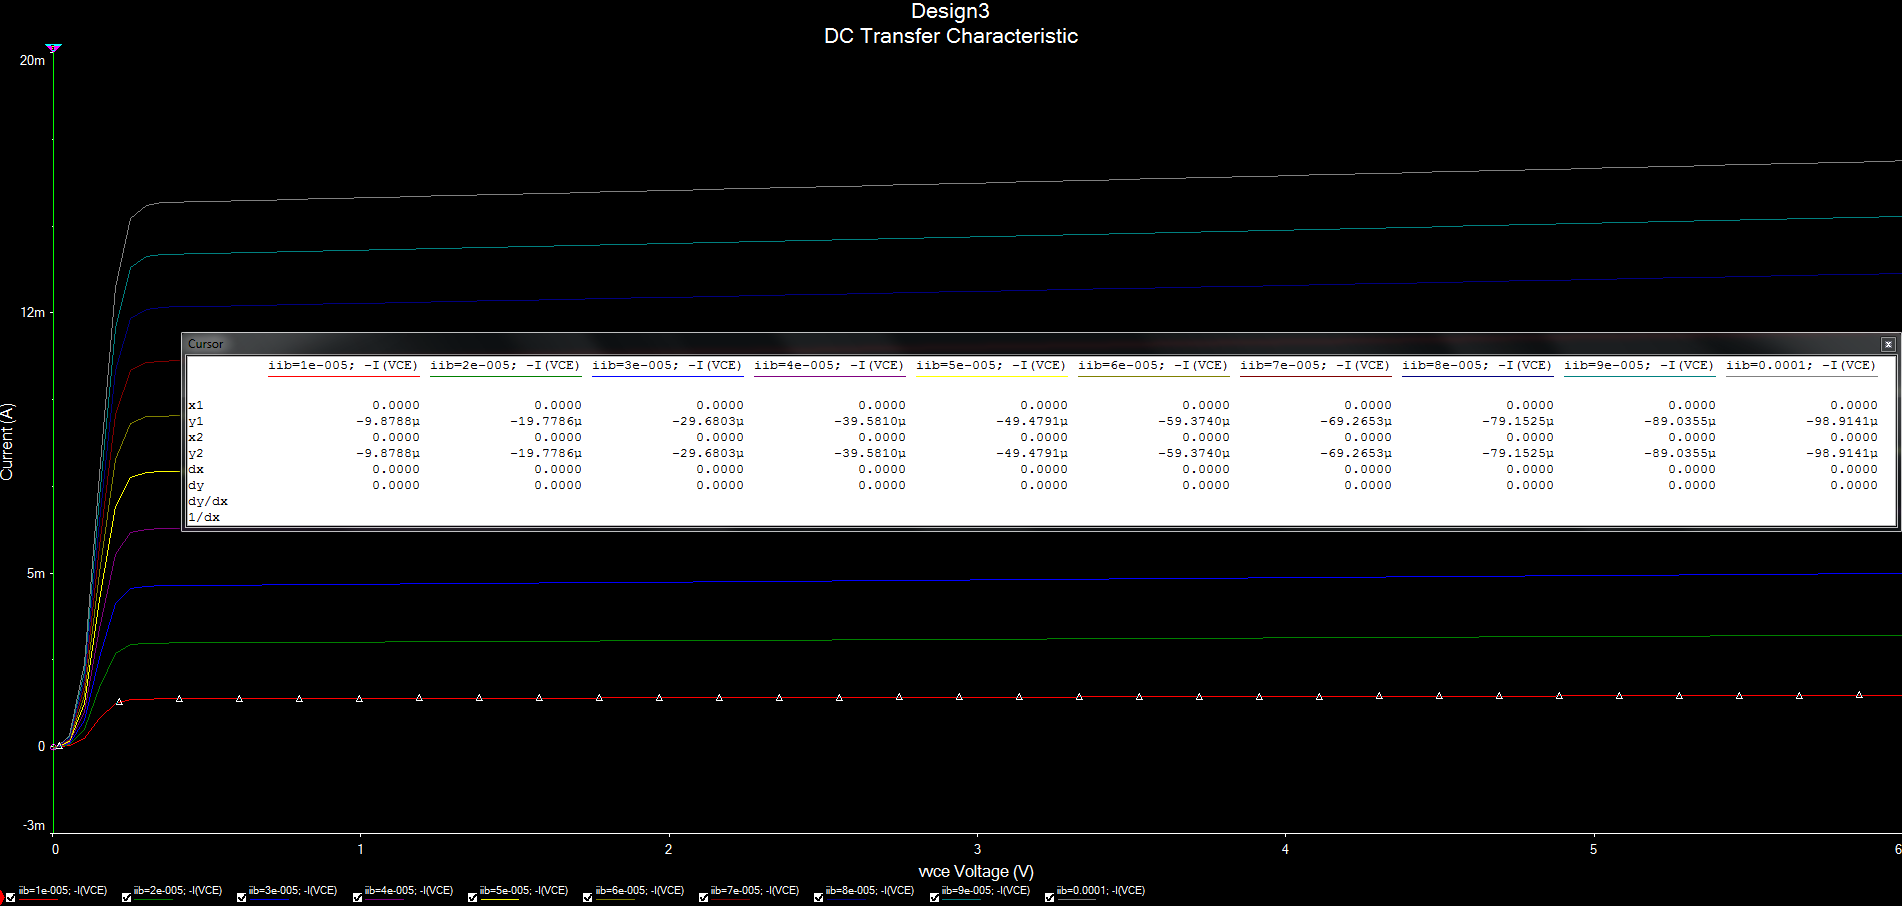
\includegraphics[height=3in]{/home/owner/Desktop/LAB REPORTS/D1/Pic7.PNG}
	\caption[A.2 Part.7 Plot]{A.2 Part.7}
	\label{fig:pic}
\end{figure}


\subsection{B:Resistevely Loaded BJT Inverter Characteristics}

\begin{figure}[H]
	\centering
	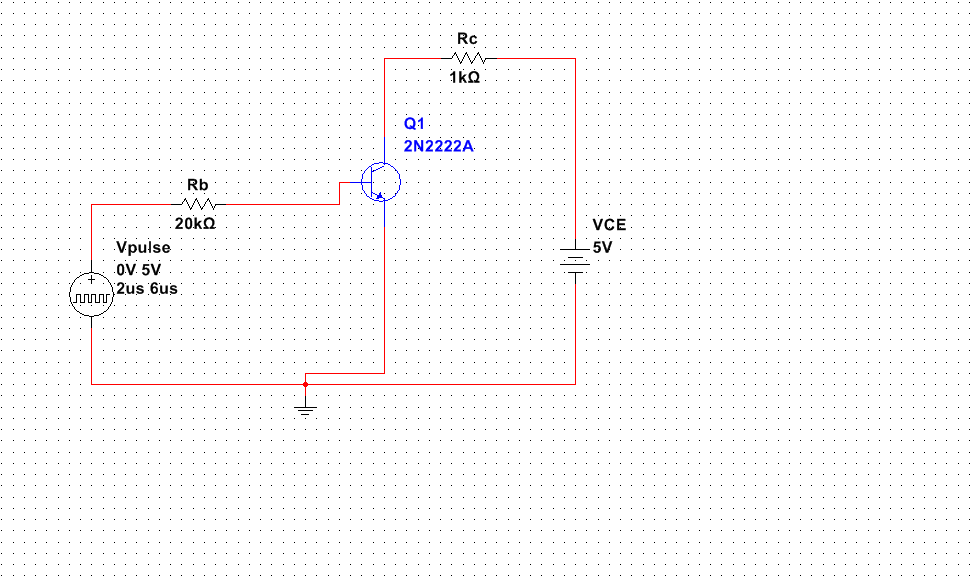
\includegraphics[height=3in]{/home/owner/Desktop/LAB REPORTS/D1/Pic8.PNG}
	\caption[B Part.3 electronic set-up]{B Part.3}
	\label{fig:pic}
\end{figure}


\begin{table}[H]
	\centering
	\label{tab:fifthTable}
	\caption[B Part.6 Table]{B Part.6 }
	\begin{tabular}{lcr}
		Voh&5V \\ \hline
		Vil max&0.53V\\ \hline
		Vol&0.3V\\ \hline
		Vih min&1.1V\\ \hline
	\end{tabular}
\end{table}


$$Voh=Vcc=5V$$

$$Vol=Vcesat=0.3V$$

$$Vil max=Vbe cut-in=0.53V$$

$$Vih min = Vbe on + \frac{Rb}{Bf*Rc}[Vcc-Vcesat]=1.1V$$

B Part.8\\
Q. Predict what will happen if Rc is increased from 1kOhm to 4kOhm.\\
Ans. The wave form will decay quicker and a steeper decline will be noticed in the wave.


\begin{figure}[H]
	\centering
	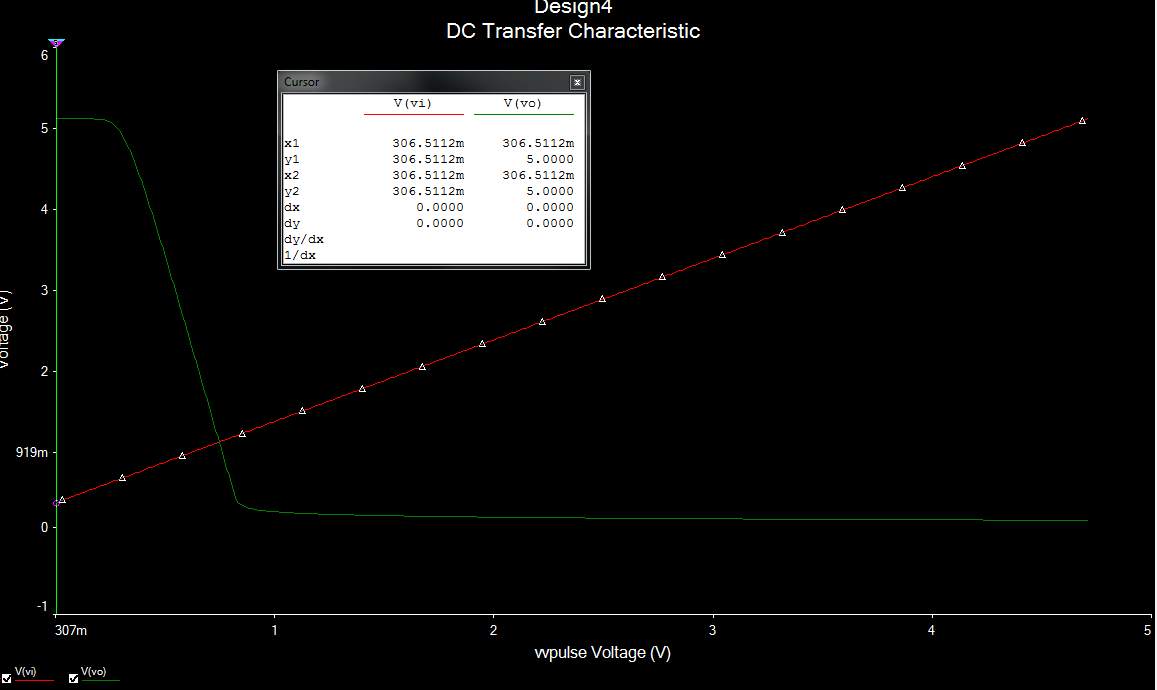
\includegraphics[height=3in]{/home/owner/Desktop/LAB REPORTS/D1/Pic9.PNG}
	\caption[B Part.9 Plot]{B Part.9}
	\label{fig:pic}
\end{figure}

\subsection{C:BJT Inverter Switching Performance}

\begin{figure}[H]
	\centering
	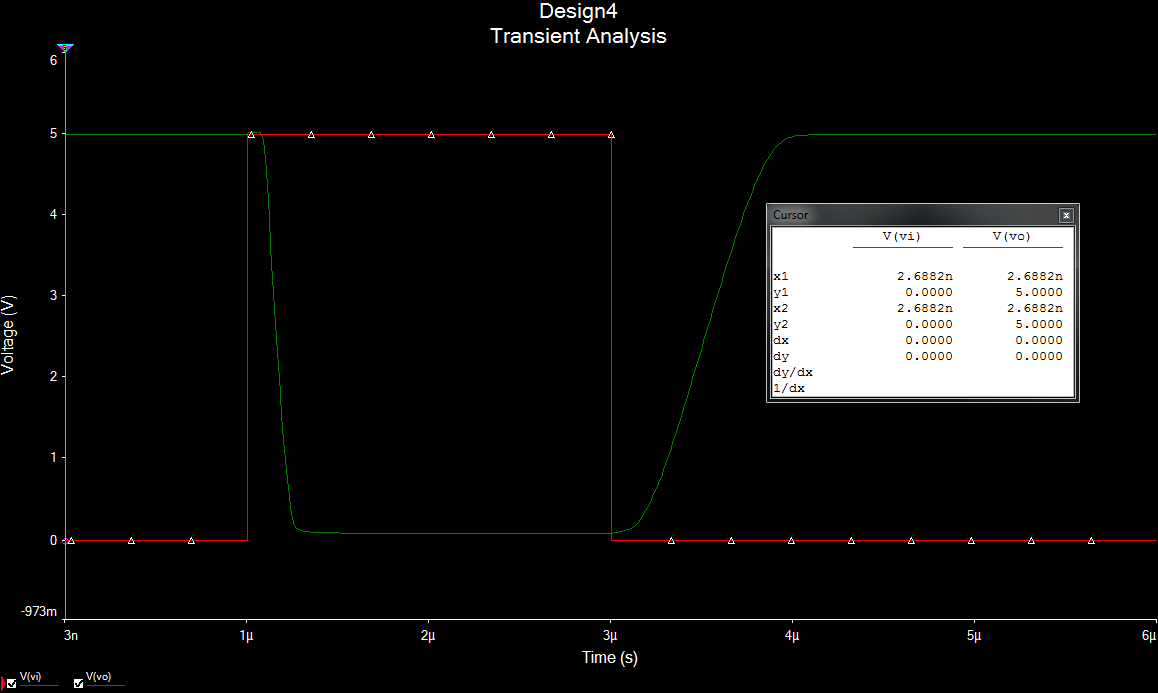
\includegraphics[height=3in]{/home/owner/Desktop/LAB REPORTS/D1/Pic10.PNG}
	\caption[C Part.2 Plot]{C Part.2}
	\label{fig:pic}
\end{figure}


\begin{table}[H]
	\centering
	\label{tab:sixthTable}
	\caption[C Part.2 Table]{C Part.2}
	\begin{tabular}{lcr}
		td&$1.5*10^{-7}s$ \\ \hline
		tf&$1.3*10^{-7}s$ \\ \hline
		ts&$1.3*10^{-7}s$ \\ \hline
		tr&$6*10^{-7}s$ \\ \hline

	\end{tabular}
\end{table}

$$td=Rb(Cje+Cjc)ln\frac{Vcc}{Vcc-Vbe cutin}=$$\\

$$td=20000(27*10^{-12}+9.12*10^{-12})ln\frac{5}{5-0.53}=8*10^{-8}s$$\\

$$tf=0.8Bf(Tf+Rc*Cjc)ln\frac{Bf*Ibf}{Bf*Ibf-Icmax}=$$ \\

$$tf=0.8*220(0.325*10^{-9}+1000*9.12*10^{-12})ln\frac{220*2.165*10^{-4}}{220*2.165*10^{-4}-4.7*10^{-3}}=1.73*10^{-7}s$$\\

$$Ibf=\frac{Vi-Vbeon}{Rb}$$\\

$$Ibf=\frac{5-0.67}{20000}=2.165*10^{-4}A$$\\

$$Ic max=\frac{Vcc-Vce sat}{Rc}$$\\

$$Ic max=\frac{5-0.3}{1000}=4.7*10^{-3}A$$\\

$$ts=ts ln\frac{Ibf-Ibr}{\frac{Icmax}{Bf} -Ibr}$$\\

$$ts=3.927*10^{-7} ln\frac{2.165*10^{-4}-(-3.35*10^{-5})}{\frac{4.7*10^{-3}}{220} -(-3.35*10^{-5})}=5.96*10^{-7}s$$\\

$$Ibr=- \frac{Vbeon}{Rb}$$\\

$$Ibr=- \frac{0.67}{20000} = -3.35*10^{-5}A$$\\


$$Ts=\frac{(1+Br)Tbf+Bf*Tbr}{1+Bf+Br}=\frac{(1+Br)Bf*Tf+Br*Bf*Tr}{1+Bf+Br}$$ \\

$$Ts=\frac{(1+Br)Tbf+Bf*Tbr}{1+Bf+Br}=\frac{(1+4)220*0.325*10^{-9}+4*220*100*10^{-9}}{1+220+4}=3.927*10^{-7}$$ \\

$$tr=0.8*Bf*(Tf+Rc*Cjc) ln\frac{\frac{Icmax}{Bf} -Ibr}{-Ibr}$$\\

$$tr=0.8*220*(0.325*10^{-9}+1000*9.12*10^{-12}) ln\frac{\frac{4.7*10{-3}}{220} -3.35*10{-5}}{-3.35*10{-5}}=8.2*10^{-7}s $$\\


\begin{table}[H]
	\centering
	\label{tab:seventhTable}
	\caption[C Part.3 Table]{C Part.3}
	\begin{tabular}{lcr}
		td&$8*10^{-8}s$ \\ \hline
		tf&$1.73*10^{-7}s$\\ \hline
		ts&$5.96*10^{-7}s$\\ \hline
		tr&$8.2*10^{-7}s$\\ \hline
	\end{tabular}
\end{table}

C Part.4
Q. Predict what will happen if Rb is reduced to 5kOhm.\\
Ans. A decrease in Rb will effect all 4 cycle times and thus when a time is divided by Rb it will increase. The increse will make the wave function apear less square therefore the drop off point will look less pronounced and the transition time will thus increase.


\begin{table}[H]
	\centering
	\label{tab:eigthTable}
	\caption[C Part.5 Table]{C Part.5}
	\begin{tabular}{lcr}
		td&$2*10^{-8}s$\\ \hline
		tf&$4*10^{-8}s$\\ \hline
		ts&$2.5*10^{-7}s$\\ \hline
		tr&$2*10^{-7}s$\\ \hline

	\end{tabular}
\end{table}


\begin{figure}[H]
	\centering
	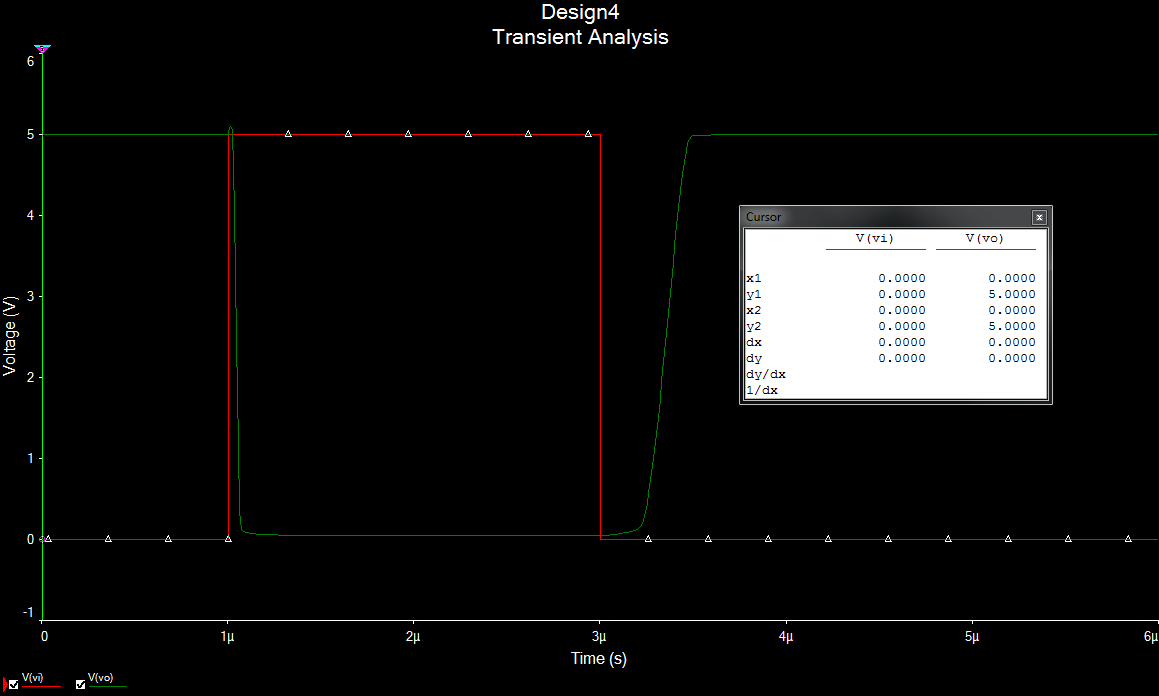
\includegraphics[height=3in]{/home/owner/Desktop/LAB REPORTS/D1/Pic11.PNG}
	\caption[C Part.5 Plot]{C Part.5}
	\label{fig:pic}
\end{figure}
\pagebreak
C Part.6
Q. Predict what will happen if Rc is increased to 4kOhm.\\
Ans. Since Rc is responsible for the value of ICmax a higher value for Rc will mean a decreased value of ICmax thus giving a smaller value for every time across the board except for td  since it is not effected by ICmax  or Rc. The drop off point will also become steeper as Vce is raised giving it a square wave look(but not turning it into a square wave ).




\begin{table}[H]

	\centering
	\caption[C Part.7 Table]{C Part.7}
	\begin{tabular}{lcr}
		td&$1*10^{-8}s$ \\ \hline
		tf&$3*10^{-8}s$\\ \hline
		ts&$2.5*10^{-7}s$\\ \hline
		tr&$2*10^{-7}s$\\ \hline

	\end{tabular}
\end{table}


\begin{figure}[H]
	\centering
	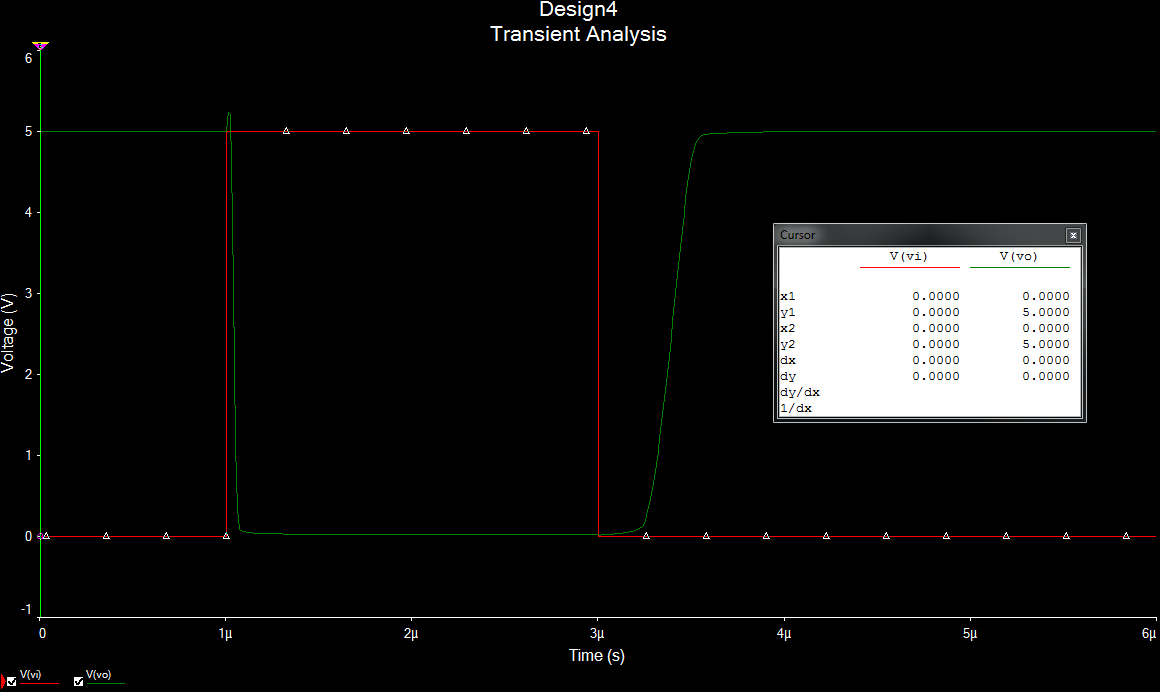
\includegraphics[height=3in]{/home/owner/Desktop/LAB REPORTS/D1/Pic12.PNG}
	\caption[C Part.7 Plot]{C Part.7}
\end{figure}


\pagebreak


\section{Discussion}\label{sec:discuss}\underline{•}
(i) What are the limitations on the accuracy of your results?\\
Human error played a big part in discerning the results as subjective viewing was used more than a real form of accurate measurement. Rounding the results also could have led to a small discrepancy between the calculated and observed results.\\
(ii) How do the values of parameters compare with those obtained in lectures?\\
In our simulation we noticed that the lines in the transient analysis were not perfectly horizontal.
	The values differed somewhat from those obtained in lectures as the values and diagrams given in lectures represent an ideal state.The Multisim plots tend to lie somewhere in between the ideal state and real world values .\\
(iii) What are the advantages or disadvantages of circuit simulations such as the one carried out in the experiment?\\
	The advantages of this simulation were that 3 distinct circuits could be simulated and analysed in a 3hour lab. If were to build the circuits manually it would have taken up substantially more time and resources.
\\
The disadvantages of this simulation is that it lacks the real world aspect of dealing with bipolar transistors. In theory someone can know how to calculate and analyse a bipolar transistor without ever having to know what it looks like which for field associated work may be a huge disadvantage. 
\\
(iv) What are the benefits or drawbacks of circuit simulation and of MultiSim in general as applied to the design of electronic circuits?
\\
The advantages of simulating an electric circuit are of course that it saves time and effort. Along with the usual advantages a simulation also allows for quicker modifications of circuit designs and instantaneous simulation of that circuit with a graph. 

	The disadvantages of the MultiSim simulations are that our virtual environment does not factor in environmentally dependent errors such as temperature and humidity. As we all know heat increases resistance .Thus the simulation can only show how a circuit will behave in ideal conditions but not in adverse ones.
\\
(v)	What are the essential elements of good circuit simulation and simulators?
\\
A good simulator should be comprised of a large library of components to choose from and be able to experiment and simulate multiple circuits quickly and efficiently. All the models in the simulation should be accurate and up to date with standard industry components. 
\\
(vi) What is the role of the Electronic Engineer in this regard?
\\
	The role of an Electronic Engineer in this regard is to design and develop the electronic circuit. The engineer must take the pre-requisite demands the circuit must fulfill and the space required for those components to fit in the wider application into consideration. Finally the role of the engineer is to understand and pre-plan for events and circumstances Multisim cannot encompass such as extreme environmental factors.


\pagebreak

\section{Conclusion}
BJT's have their limitations, but given their wide potential and current applications in electronics, the conclusion drawn from completing this laboratory is that the BJT is an important piece in the world of semiconductors.	
	Although there were discrepancies between the Multisim values and the real world values, multisim has proven a very fast and relatvelly accurate way of designing and testing electronic circuits encompassing BJT's.\\
	
	



\appendix
\section{References}
This is a list of links used for further information.

	\begin{enumerate}
	
		\item http://fourier.eng.hmc.edu/e84/lectures/ch4/node3.html
		\item http://aries.ucsd.edu/NAJMABADI/CLASS/ECE65/06-W/NOTES/BJT1.pdf
		\item The Art of Electronics-Paul Horowitz and Winfield Hill
		\item Solid State Electronic Devices, Sixth Edition pg.251
		\item Solid State Electronic Devices, Sixth Edition pg.363
		\item http://www.allaboutcircuits.com/textbook/semiconductors/chpt-4/transistor-switch-bjt/
		
		
	\end{enumerate}


\end{document}